%% Machine Learning: Science and Technology (MLST, IOP Publishing) submission
%% Class: iopart.cls; reference style: iopart-num (numeric).
%% iopart.cls and iopart-num.bst are bundled by Overleaf's IOP template;
%% if compiling locally, obtain them from CTAN (package "iopart").

\documentclass[12pt]{iopart}

%%%% Packages
\usepackage[T1]{fontenc}%   % accented letters in bibliography (e.g. Rozpędek)
\usepackage{lmodern}%       % T1-aware Computer Modern
% amsmath, amssymb, and bm are loaded through iopams below.
\usepackage{graphicx}%
\usepackage{booktabs}%
\usepackage{xcolor}%
\usepackage{braket}%        % \bra, \ket
\usepackage{enumitem}%      % list option keys
\usepackage{iopams}%        % IOP AMS/bm support (loads amsmath, amssymb, bm)
\usepackage[capitalize]{cleveref}%
\providecommand{\tfrac}[2]{\frac{#1}{#2}}
\providecommand{\eqref}[1]{(\ref{#1})}
\providecommand{\bm}[1]{\boldsymbol{#1}}
\providecommand{\binom}[2]{{#1\choose #2}}
\usepackage{url}%

%%%% Project-specific shorthands
\newcommand{\Fe}{F_{\mathrm{e}}}
\newcommand{\Fhat}{\widehat{F}}
\newcommand{\Fehat}{\widehat{F}_{\mathrm{e}}}
\newcommand{\Choi}{\mathcal{J}}
\newcommand{\Lset}{\Lambda}
\newcommand{\eps}{\varepsilon}
\newcommand{\dnorm}{\diamond}
\newcommand{\fidno}{\textsc{FidelityFormer}}
\newcommand{\dfe}{\textsc{DFE}}
\newcommand{\eg}{\textit{e.g.}}
\newcommand{\ie}{\textit{i.e.}}

\graphicspath{{figures/}}

\begin{document}

\title[Information-limited fidelity estimation]{Information-limited fidelity estimation of composed quantum channels: when to compose, measure, or learn}

\author{Shuchang Wang$^{1,\dagger}$, Xiaoman Liu$^{1,\dagger}$ and Wei Yang$^{1}$}

\address{$^{1}$ School of Computer Science and Technology, University of Science and Technology of China, Hefei 230026, China}

\ead{qubit@ustc.edu.cn}

\begin{abstract}
Scientific machine-learning estimators are meaningful only relative to the information and measurement budget available at inference. We make this information contract explicit for end-to-end entanglement fidelity of composed quantum channels. Two negative controls delimit the problem: with complete Markovian Choi descriptions, deterministic superoperator composition is numerically exact and faster than the learned models at the studied dimensions; with access to the deployed process, stratified Direct Fidelity Estimation (DFE) is a strong low-shot baseline. The non-trivial case is a collision process observed only through reset-bath marginal channels. We define a representation ambiguity diameter and prove that half this diameter lower-bounds the worst-case error of every estimator using that representation. Counterfactual replay of 2048 collision sequences across 15 indistinguishable bath-retention values gives mean diameter $0.229$, a mean pointwise minimax lower bound $0.115$, and a Bayes MAE floor $0.060$ under a uniform high-memory prior. This certificate motivates a measurement-conditioned estimator that convexly fuses a calibrated marginal prior with a same-query DFE pilot. On a fresh 4096-sample split generated with independent parameter and retention random streams, a 32-shot neural hybrid reaches MAE $0.0657$, matching 64-shot DFE ($0.0641$); at 64 shots it reaches $0.0539$, matching 96-shot DFE ($0.0525$). Including finite-shot labels and fusion fitting, the corresponding offline costs amortise after 192 and 256 deployment queries. The contribution is therefore not another universally superior architecture, but a testable procedure for detecting when inputs are insufficient and for buying back the missing information with a small, explicitly costed measurement budget.
\end{abstract}

\vspace{1pc}
\noindent{\it Keywords}: information-limited learning, scientific machine learning, quantum channels, fidelity estimation, identifiability, non-Markovian dynamics

\vspace{1pc}
\noindent$^{\dagger}$ These authors contributed equally to this work.


%%%% BEGIN flattened: sections/01_introduction
\section{Introduction}
\label{sec:intro}

A learned scientific estimator should be judged against what is observable at inference, not only against other architectures. If the supplied variables already determine the target, a deterministic computation is preferable. If they do not, no architecture can reconstruct instance-specific missing information without an additional observation or assumption. This distinction is especially important for composed quantum channels, where per-step channel descriptions, classical simulators, and measurements of the deployed process expose different information.

We study the end-to-end entanglement fidelity $\Fe$ of a channel sequence. The quantity appears in repeater and purification design~\cite{repeater_review,dur2007entanglement}, validation of NISQ circuits~\cite{nisq_validation}, and fidelity-based screening in quantum-error-correction workflows~\cite{qec_review}. Common estimators occupy distinct information--cost regimes. Products of marginal fidelities and Kraus-path Monte Carlo use only per-step channel descriptions. Exact superoperator composition is available when those descriptions fully specify a Markovian process. Direct Fidelity Estimation (DFE)~\cite{flammia_liu_2011} instead measures the deployed composed channel. A learned sequence model can amortise computation or prior characterisation, but it cannot evade missing-variable ambiguity.

This paper turns that observation into an empirical and mathematical audit. Our decisive setting is a non-Markovian collision process whose inputs are reset-bath marginal Choi matrices while the target is produced by joint system--bath propagation. The bath-retention variable $\eta$ is deliberately omitted. Counterfactual replay can therefore hold every supplied input fixed while varying $\eta$, producing a fibre of different valid targets. We quantify the resulting representation ambiguity, derive estimator-independent lower bounds, and compare actual predictors with those bounds. This separates model error from irreducible error caused by the information contract.

The ambiguity certificate also suggests a constructive response. Rather than choosing between a zero-shot prior and a measurement-only estimator, we fit a constrained convex fusion of the marginal prediction and a low-shot DFE estimate made on the same query. The prior dominates when the pilot is noisy; the measurement receives increasing weight as its budget grows. All calibration labels and pilot measurements are simulated with independent binomial outcomes, and their offline cost is included. A fresh OOD dataset uses independent random streams for collision parameters and $\eta$, ruling out random-number coupling as an explanation.

We retain broad negative controls. In hardware-like Markovian and two-qubit regimes, exact composition or classical Monte Carlo can dominate the neural models. In the collision regime, enumerating all four Pauli settings makes DFE much stronger than a settings-with-replacement implementation. These controls narrow, rather than inflate, the learned method's claim.

Our contributions are:
\begin{enumerate}[label=(\alph*),itemsep=2pt,topsep=2pt]
\item We formalise a representation-dependent ambiguity diameter for composed-channel fidelity and derive worst-case and distributional MAE lower bounds that apply to every estimator using the same inputs.
\item We introduce a paired counterfactual collision audit. Across 2048 fixed marginal inputs and 15 high-memory values, it measures a mean ambiguity diameter of $0.229$ and a Bayes MAE floor of $0.060$.
\item We develop a measurement-conditioned prior--DFE fusion rule with an explicit finite-shot calibration contract. It approximately halves the per-query shots needed to reach MAE $\simeq0.065$ and reduces them by one third near MAE $\simeq0.053$.
\item We provide exact-composition, low-capacity, Monte-Carlo, stratified-DFE, independent-random-stream, and full amortised-cost controls, yielding a practical rule for when to compose, measure, learn, or combine them.
\end{enumerate}
The novelty lies in diagnosing and repairing information insufficiency, not in claiming universal superiority for a particular neural architecture.

% \paragraph*{Outline.}% \paragraph*{Outline.}
% \Cref{sec:setup} fixes notation and defines the three regimes. \Cref{sec:arch} describes the \fidno{} architecture and the recalibration step. \Cref{sec:baselines} lists baselines. \Cref{sec:experiments} reports experiments and the \dfe{} crossover. \Cref{sec:operating} derives the operating-regime decision rule and discusses QEC compatibility without making a decoder claim. \Cref{sec:related,sec:conclusion} cover related work and conclude.
%%%% END flattened: sections/01_introduction


%%%% BEGIN flattened: sections/02_setup
\section{Setup}
\label{sec:setup}

\subsection{Channel sequences and entanglement fidelity}

Let $\mathcal{H}_S$ be a finite-dimensional system Hilbert space with dimension $d$. A quantum channel is a completely positive trace-preserving (CPTP) map
$\Lset : \mathcal{B}(\mathcal{H}_S) \to \mathcal{B}(\mathcal{H}_S)$. For an ordered sequence $\Lset_1,\ldots,\Lset_n$, we write
$\Lset_{1:n} \equiv \Lset_n \circ \cdots \circ \Lset_1$.
We use the unnormalised Choi--Jamiolkowski matrix~\cite{choi75,jamiolkowski72}
\begin{equation}
\Choi(\Lset) \;=\; \sum_{i,j=0}^{d-1}
\ket{i}\!\bra{j} \otimes \Lset\bigl(\ket{i}\!\bra{j}\bigr)
\in \mathcal{B}(\mathcal{H}_S \otimes \mathcal{H}_S),
\end{equation}
which obeys $\Choi(\Lset) \succeq 0$, $\mathrm{Tr}[\Choi(\Lset)] = d$, and
$\mathrm{Tr}_{2}[\Choi(\Lset)] = \mathbb{1}_{S}$ for every CPTP map.

The prediction target is the entanglement fidelity~\cite{schumacher96} of a channel with respect to the identity,
\begin{equation}
\Fe(\Lset) \;=\; \frac{1}{d^{2}}
\mathrm{Tr}\bigl[\Choi(\mathrm{id})^{\dagger} \Choi(\Lset)\bigr]
\;=\;
\langle \Phi^{+} |
(\mathrm{id} \otimes \Lset)(|\Phi^{+}\rangle\!\langle\Phi^{+}|)
| \Phi^{+} \rangle,
\label{eq:Fe_def}
\end{equation}
where $|\Phi^{+}\rangle = d^{-1/2} \sum_i |ii\rangle$.
We use $\Fe$ rather than the average gate fidelity
$F_{\mathrm{avg}} = (d \Fe + 1)/(d+1)$ because it is the target of our downstream estimates and of \dfe.

The composed-channel prediction problem is
\begin{equation}
\fidno_{\theta}: \quad
\bigl(\Choi(\Lset_1), \ldots, \Choi(\Lset_n) \bigr)
\;\longmapsto\;
p_{\theta}\bigl(\Fe(\Lset_{1:n})\bigr),
\label{eq:problem}
\end{equation}
where $p_\theta$ is a calibrated distribution over $\Fe \in [0,1]$, implemented with a quantile head.

\subsection{Representation ambiguity and estimator-independent limits}
\label{sec:ambiguity}

Let $z$ denote a complete physical instance, $F(z)\in[0,1]$ its target fidelity, and $x=\phi(z)$ the representation supplied to an estimator. The fibre $\mathcal{A}_{\phi}(x)=\{z:\phi(z)=x\}$ contains all physical instances indistinguishable from the input. Define its target diameter
\begin{equation}
\Delta_{\phi}(x)=\sup_{z,z'\in\mathcal{A}_{\phi}(x)} |F(z)-F(z')|.
\label{eq:ambiguity_diameter}
\end{equation}
For any deterministic estimator $h(x)$,
\begin{equation}
\sup_{z\in\mathcal{A}_{\phi}(x)} |h(x)-F(z)|\geq \tfrac{1}{2}\Delta_{\phi}(x).
\label{eq:minimax_floor}
\end{equation}
Indeed, the triangle inequality applied to two targets approaching the fibre extrema gives $\Delta_{\phi}(x)\leq |F(z)-h(x)|+|h(x)-F(z')|$. This is a pointwise worst-case statement, not an average-MAE bound. Under a specified conditional distribution $p(F\mid x)$, the MAE-optimal predictor is a conditional median and the Bayes risk is
\begin{equation}
R^{\star}_{\phi}=\mathbb{E}_{x}\mathbb{E}_{F\mid x}
\bigl[|F-\mathop{\mathrm{median}}(F\mid x)|\bigr].
\label{eq:bayes_floor}
\end{equation}
We estimate both quantities by counterfactually replaying fixed collision parameters across a grid of hidden retention values. The supplementary material gives the protocol and proof details.

\subsection{Three operating regimes}

We evaluate the estimators in three regimes spanning more than two orders of magnitude in per-channel infidelity.

\begin{description}[itemsep=3pt,topsep=2pt,leftmargin=*]
\item[(R1) Device regime ($d{=}2$, $\eps \approx 10^{-3}$).]
Single-qubit channels are sampled from hardware-calibrated parametric noise models spanning amplitude damping, phase damping, depolarising, and Lindblad families, with parameter ranges matched to the reported single-qubit gate-error scale of current superconducting and trapped-ion processors~\cite{ibm_fake_backends}. The \texttt{family\_ood} split holds out the Pauli-channel family entirely. The per-channel infidelity is $\eps \approx 10^{-3}$, matching the hardware gate-error scale.

\item[(R2) Non-Markovian collision regime ($d{=}2$, $\eps \approx 0.4$).]
The system and a bath qubit initially in $|+\rangle$ interact through step-dependent commuting $ZZ$ Hamiltonians. After each collision the joint state is retained with probability $\eta$ and otherwise the bath is reset. Training, calibration, and ID data use $\eta\in[0,0.7]$; the legacy \texttt{family\_ood} file instead holds out the stronger interval $\eta\in[0.85,0.99]$. It is therefore a memory-strength distribution shift, not a held-out collision family.

\item[(R3) Two-qubit order-sensitive regime ($d{=}4$).]
This regime contains two-qubit channels built from correlated dephasing, two-qubit depolarising noise, and imperfect SWAP/CNOT operations with both coherent and incoherent errors. The order-sensitive variant introduces non-commutativity between consecutive channels, so order-invariant baselines such as DeepSets lose relevant information. This regime tests whether the behaviour observed at $d=2$ extends to larger systems.
\end{description}

\subsection{Splits and metrics}

Each regime is divided into \texttt{train}, \texttt{calib}, \texttt{id\_test}, \texttt{length\_ood}, and a distribution-shift split. The first three use lengths in $\{2,4,8,16\}$ and \texttt{length\_ood} uses $\{24,32,48\}$. R1 and R3 hold out a noise family; R2 holds out a high-$\eta$ memory-strength interval while retaining the legacy filename \texttt{family\_ood} for code compatibility.

The main metric is pooled MAE on $\Fe$ across five independent seed-controlled splits. We also report the MAE after post-hoc affine recalibration (\cref{app:recalibration}) and the quantum-shot cost for measurement-based estimators. Calibration metrics for the distributional outputs, including CRPS, expected calibration error (ECE), and quantile coverage, are reported in the supplementary material. Unless stated otherwise, tables report means over five seeds, with standard deviations shown alongside the neural rows; per-seed recalibration coefficients are given in the appendix.
%%%% END flattened: sections/02_setup


%%%% BEGIN flattened: sections/03_architecture
\section{Architecture}
\label{sec:arch}

\subsection{Choi-aware per-channel encoder}

Each channel $\Lset_i$ enters the model through its Choi matrix $\Choi(\Lset_i) \in \mathbb{C}^{d^2 \times d^2}$. The Choi representation preserves CPTP structure (positivity and the partial-trace constraint) exactly, unlike a flattened superoperator. We Hermitian-symmetrise $\Choi(\Lset_i) \to \tfrac{1}{2}\bigl(\Choi(\Lset_i) + \Choi(\Lset_i)^{\dagger}\bigr)$ and split the result into real and imaginary parts, yielding $2 d^{4}$ real numbers per channel ($32$ for $d{=}2$, $512$ for $d{=}4$). The imaginary block is anti-symmetric and therefore formally over-parameterised; we retain it for code simplicity and let the encoder learn the redundancy. A two-layer MLP (multi-layer perceptron) with width $D = 256$ and GELU activations maps the vector to a channel token $z_i \in \mathbb{R}^{D}$. As an ablation we provide a Pauli-transfer-matrix (PTM) variant of the encoder, which produces $d^{4} = 16$ real numbers per channel at $d{=}2$. Supplementary Sec.~S4 finds PTM and Choi encoders statistically indistinguishable on the collision regime, with differences below $0.003$ pooled MAE on all three splits and within seed noise.

\subsection{Causal transformer backbone}

A depth-$6$ causal transformer with $h = 8$ heads, $d_{\mathrm{model}} = D = 256$, FFN expansion $4\times$, and rotary positional encoding then processes the channel tokens $z_1, \ldots, z_n$. Causal masking blocks the position-$i$ token from attending to later channels, which we find beneficial for stable length-OOD behaviour: bidirectional attention overfits the within-distribution length distribution and tends to degrade faster on extrapolation, even though it slightly outperforms causal attention on $\texttt{id\_test}$ and the two variants are close on the calibrated OOD splits (\cref{sec:experiments}). We adopt causal masking because it matches the sequential composition structure and is the more stable default, not because it is uniquely required.

\subsection{Quantile distribution head}

The pooled sequence representation feeds two heads. The primary head produces $K = 9$ quantile predictions at nominal levels $\{0.1, 0.2, \ldots, 0.9\}$, trained with the pinball (quantile-regression) loss
\begin{equation}
\mathcal{L}_{\mathrm{pinball}} \;=\; \sum_{k=1}^{K} \rho_{q_k}\!\bigl( \Fe^{\mathrm{true}} - \Fhat_{q_k} \bigr),
\label{eq:pinball}
\end{equation}
with $\rho_{q}(u) = u(q - \mathbb{1}[u<0])$. We initialise the median-quantile head bias so that the softplus output starts at $\Fe \approx 0.7$; without this initialisation the head saturates into a dead-gradient region within the first few hundred steps when fitting the deep-circuit regime. As an ablation, we also implement a Gaussian head outputting $(\mu, \log\sigma)$ trained with truncated-normal NLL.

\subsection{Auxiliary physics-consistency loss}

We attach a small auxiliary head (weight $\lambda_{\mathrm{aux}}=0.1$) that predicts the purity $\mathrm{Tr}[\Choi^2]/d^{2}$ of the composed Choi, intended to encourage internal representations that separate unitary from heavily decoherent compositions. The auxiliary head does not affect point-prediction MAE on the collision regime ($\lambda_{\mathrm{aux}} \in \{0, 0.1\}$ match within seed noise on all three splits); consistent with the theme of this paper, no single architectural component is decisive, and the Choi-aware encoder and causal backbone are best understood as reasonable, stable defaults rather than as the source of the effect. Full design and the ablation are in the supplementary material; the head is removed at inference.

\subsection{Post-hoc affine recalibration}
\label{sec:recal}

Distribution shift between training and OOD splits manifests as a near-affine bias in the predicted median: $\Fhat^{\mathrm{raw}}_{q_{0.5}} \approx a^{-1} (\Fe^{\mathrm{true}} - b)$ over the OOD population. We exploit this with a one-line correction
\begin{equation}
\Fhat^{\mathrm{cal}}_{q_{0.5}} \;=\; a \cdot \Fhat^{\mathrm{raw}}_{q_{0.5}} + b,
\label{eq:recal}
\end{equation}
where $(a, b)$ are fitted by ordinary least squares on a labelled OOD calibration set disjoint from the test set. Our headline configuration uses $N_{\mathrm{cal}} = 64$ because the calibration-size sweep saturates at $N_{\mathrm{cal}} \in \{64, 128\}$ (the supplementary material reports the full sweep down to $N_{\mathrm{cal}} = 8$). We call this the \emph{labelled-OOD calibration} setting: the test set sees no labels at inference, but a labelled OOD calibration set is assumed available offline. Synthetic labels are generated by the corresponding exact simulator: Choi/superoperator composition for the Markovian regimes and joint system--bath propagation for the collision regime. In an experimental deployment they would have to come from an offline labelled characterisation campaign, such as \dfe{} or tomography on representative OOD instances, and their quantum or classical cost must be amortised over subsequent deployment queries. The result is zero \emph{per-query} measurement cost after calibration, not unconditional zero-shot learning.

We use a linear rather than isotonic, conformal, or non-linear correction because the residual after subtracting $(a, b)$ from the raw predictions is small relative to the OOD bias (\cref{app:recalibration}). The same correction is applied at every quantile level for the distributional output.

Across five seeds, the raw $(a, b)$ vary by std $\approx 0.09$, but the post-calibration MAE varies by only $1.3 \times 10^{-3}$, a factor of $\approx 70$ smaller than the bias correction itself (\cref{app:recalibration}). The seeds reach the same calibrated MAE along several distinct affine paths, indicating that the OOD bias is structural rather than seed noise.
%%%% END flattened: sections/03_architecture


%%%% BEGIN flattened: sections/04_baselines
\section{Baselines}
\label{sec:baselines}

We compare \fidno{} with analytic estimators, measurement-based estimators, classical Monte-Carlo sampling, and neural alternatives.

\subsection{Analytic baselines}

\paragraph*{Product approximation.}
The primary analytic baseline is
\begin{equation}
\Fhat_{\mathrm{prod}}=\prod_i \Fe(\Lset_i),
\label{eq:product_approx}
\end{equation}
computed directly from the per-channel Choi matrices. It uses only marginal channel information and requires no quantum measurements.

\paragraph*{Exact composition of observed channels.}
When full per-step Choi matrices are supplied and the process is Markovian, their superoperators can be multiplied deterministically and the target fidelity evaluated exactly. We include this baseline and its wall-clock cost. In R2 it composes only the reset-bath marginals, so its residual error measures the information missing from those inputs.

\paragraph*{Fuchs--van de Graaf bound.}
We also use a conservative estimator derived from the relation between fidelity and Choi trace distance,
\[
\Fe \geq 1-\frac{1}{2}\|\mathrm{id}-\Lset\|_{1,1}.
\]
Per-channel infidelities are propagated through a sub-additive composition rule to obtain a one-sided lower bound on the composed-channel fidelity. We report its MAE as a point predictor to quantify how well this cheap analytic lower bound tracks the true $\Fe$.

\paragraph*{Diamond-norm SDP.}
As a stronger analytic baseline, we solve the Watrous diamond-norm SDP~\cite{watrous_dnorm_sdp} for the marginal-composed channel and convert the result using
\[
\Fe \geq 1-\tfrac{1}{2}\|\mathrm{id}-\Lset\|_{\diamond}.
\]
The SDP is solved with SCS through \texttt{cvxpy}~\cite{cvxpy} and the QuTiP wrapper~\cite{qutip}. Like the product approximation, this baseline uses the marginal-composed channel, not the true non-Markovian composed process.

\subsection{Measurement and sampling baselines}

\paragraph*{Direct Fidelity Estimation~\cite{flammia_liu_2011}.}
\dfe{} estimates $\Fe(\Lset_{1:n})$ by measuring Pauli observables on the deployed composed channel. For the single-qubit identity target all four Pauli settings have nonzero relevance. Sampling those settings with replacement adds avoidable protocol variance once the requested number of settings exceeds four. We therefore enumerate the support, allocate a fixed total shot budget across it in proportion to the square root of the target relevance, and simulate exact binomial $\{+1,-1\}$ outcomes. We report total projective shots per sequence, sweeping 4--2000 shots in R2.

\paragraph*{Measurement-conditioned prior--DFE fusion.}
The ambiguity result implies that a marginal-only predictor cannot resolve the hidden memory of an individual query. We therefore combine a calibrated marginal prior $h_{\phi}(x)$ with an independent $B$-shot DFE pilot $\widehat F_{\mathrm{DFE},B}$ on that same query:
\begin{equation}
\widehat F_{\mathrm{hyb},B}=\mathop{\mathrm{clip}}_{[0,1]}
\left[(1-w_B)h_{\phi}(x)+w_B\widehat F_{\mathrm{DFE},B}\right],
\qquad 0\leq w_B\leq1.
\label{eq:hybrid}
\end{equation}
The scalar $w_B$ is fitted by least squares on 64 OOD calibration instances. In the realistic setting, their targets are independent 64-shot DFE estimates, while separate $B$-shot outcomes fit $w_B$. The one-time quantum cost is therefore $64\times64+64\times B$ shots, and deployment costs $B$ shots per query. We evaluate neural, summary-ridge, and exact-marginal priors under the identical protocol.

\paragraph*{Monte-Carlo Kraus sampling.}
This classical baseline samples $K$ Kraus paths from the per-channel marginal channels, propagates the maximally entangled state along each path, and averages the resulting fidelities~\cite{wood_kraus_mc}. We sweep
$K \in \{10,100,1000\}$. Since the sampling distribution is built from marginal channels, this estimator is blind to correlations carried by a shared bath.

\paragraph*{Randomized benchmarking.}
Randomized benchmarking~\cite{rb_review} is not included in the direct cost-accuracy comparison because it estimates average gate fidelity from twirled Clifford sequences rather than the entanglement fidelity of a fixed arbitrary composed channel. Its cost is also tied to decay-curve estimation rather than to a per-sequence query model. We discuss its relationship to our setting in~\cref{sec:related}.

\subsection{Neural baselines}

We train four neural alternatives using the same data, channel encoder, distribution head, optimiser, schedule, and seed list as \fidno{}.

\begin{description}[itemsep=2pt,topsep=2pt,leftmargin=*]
\item[MLP.]
A positional MLP that concatenates the Choi features from all channels and is therefore order-aware.

\item[DeepSets~\cite{deepsets}.]
An order-invariant model that sum-pools channel tokens. We include it to test whether the regime contains information that depends on channel order.

\item[BiDir Transformer.]
A transformer with the same backbone as \fidno{} but without the causal mask. This isolates the effect of causal attention.

\item[GNN.]
A linear-chain graph neural network with channel tokens as nodes and edges between consecutive channels. We use two message-passing variants, \textsc{gnn} and \textsc{generic\_gnn}, both built on the shared channel encoder.
\end{description}

All neural models are trained with AdamW, learning rate $3\times10^{-4}$, cosine decay, $80$ epochs, batch size $256$, and early-stopping patience $20$. The neural baselines differ only in sequence backbone and order handling.
%%%% END flattened: sections/04_baselines


%%%% BEGIN flattened: sections/05_experiments
\section{Experiments}
\label{sec:experiments}

We present the results by operating regime. \Cref{fig:central} gives the cost--accuracy summary, and \cref{tab:device,tab:hybrid,tab:d4} report the corresponding MAE values.

\begin{figure*}[t]
\centering
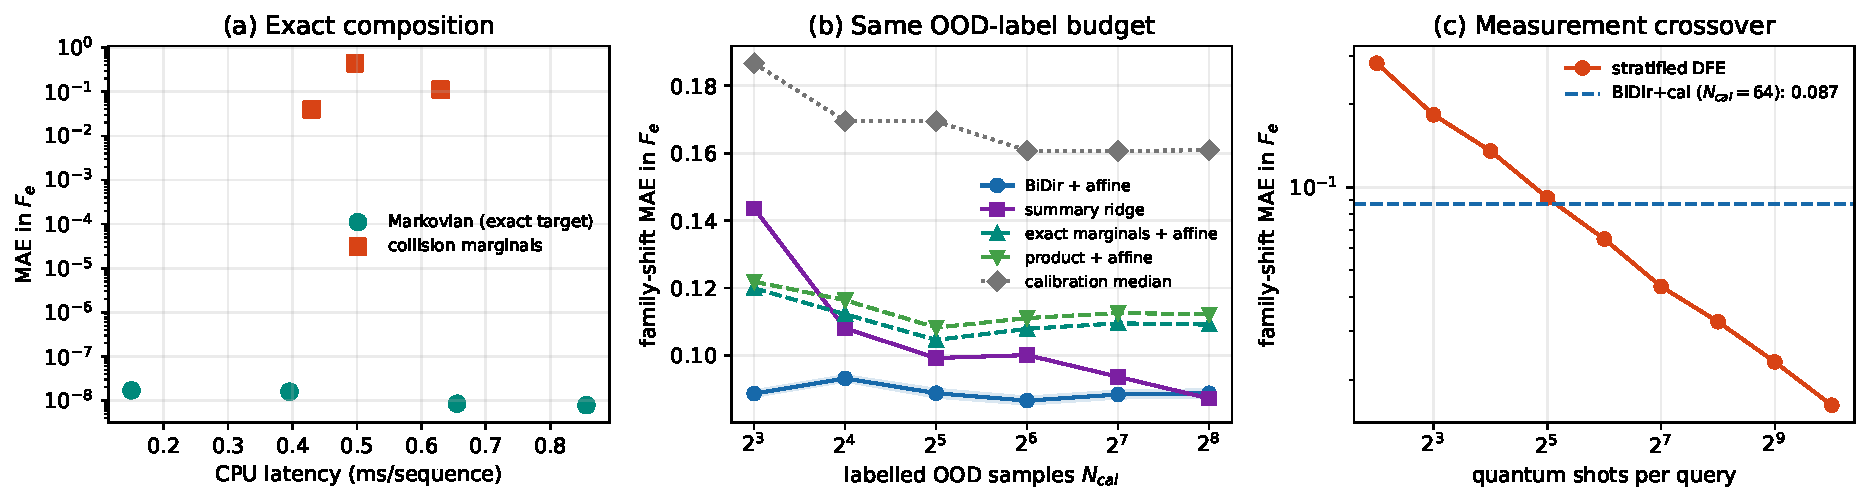
\includegraphics[width=\textwidth]{central_sample_complexity.pdf}
\caption{\textbf{Negative controls and corrected cost--accuracy comparison.}
(a) Direct composition is numerically exact on Markovian full-Choi inputs at the studied $d\leq4$ scale; collision points show the error of composing only observable reset-bath marginals. (b) All OOD-calibrated methods receive identical labelled indices. (c) Stratified DFE reaches the calibrated neural error near 32 shots per query and surpasses it at 64 shots.}
\label{fig:central}
\end{figure*}

\subsection{Device regime: hardware-realistic noise}
\label{sec:exp_device}

\Cref{tab:device} reports the device-noise regime. Because the input contains the full Choi matrix of every Markovian step, direct superoperator composition is the decisive control: its MAE is $2.4\times10^{-8}$, $4.2\times10^{-8}$, and $3.8\times10^{-8}$ on ID, length-OOD, and family-OOD, respectively, consistent with float32 feature roundoff. No learned estimator is justified when this information and computation are available. The product approximation remains the cheapest closed-form alternative and is accurate at $10^{-4}$--$10^{-3}$ scale. The near-zero marginal diamond-SDP value on family-OOD is a Pauli-geometry artefact, not a generic SDP advantage.

\begin{table}[h]
\centering
\caption{\textbf{Device regime: pooled MAE on $\Fe$.} Exact composition uses 1024 sequences per split; neural rows use five seeds and labelled-OOD calibration. The full-Choi exact baseline is limited only by stored float32 precision.}
\label{tab:device}
\small
\begin{tabular}{lccc}
\toprule
Method & \texttt{id\_test} & \texttt{length\_ood} & \texttt{family\_ood} \\
\midrule
\multicolumn{4}{l}{\emph{Deterministic and analytic, zero shots}} \\
Exact composition & $\bm{2.4\!\times\!10^{-8}}$ & $\bm{4.2\!\times\!10^{-8}}$ & $\bm{3.8\!\times\!10^{-8}}$ \\
Product approx.   & $1.0\!\times\!10^{-4}$ & $1.6\!\times\!10^{-3}$ & $2.8\!\times\!10^{-4}$ \\
FvG bound         & $3.5\!\times\!10^{-4}$ & $5.4\!\times\!10^{-3}$ & $1.2\!\times\!10^{-3}$ \\
Diamond SDP       & $1.0\!\times\!10^{-2}$ & $5.1\!\times\!10^{-2}$ & $7.8\!\times\!10^{-8}\,^{\dagger}$ \\
\midrule
\multicolumn{4}{l}{\emph{Neural, no per-query quantum measurements after labelled-OOD calibration}} \\
\fidno + cal    & $(4\!\pm\!2)\!\times\!10^{-4}$ & $(4.3\!\pm\!0.1)\!\times\!10^{-2}$ & $(1.1\!\pm\!0.2)\!\times\!10^{-2}$ \\
\textsc{mlp} + cal& $(6.8\!\pm\!0.9)\!\times\!10^{-3}$ & $(5.0\!\pm\!1.4)\!\times\!10^{-2}$ & $(1.4\!\pm\!0.6)\!\times\!10^{-2}$ \\
\textsc{deepsets} + cal & $(1.19\!\pm\!0.00)\!\times\!10^{-2}$ & $(6.4\!\pm\!0.0)\!\times\!10^{-2}$ & $(2.2\!\pm\!0.0)\!\times\!10^{-2}$ \\
\textsc{bidir} + cal    & $(7\!\pm\!2)\!\times\!10^{-4}$ & $(3.5\!\pm\!0.2)\!\times\!10^{-2}$ & $(1.5\!\pm\!0.3)\!\times\!10^{-2}$ \\
\midrule
\multicolumn{4}{l}{\emph{Measurement and sampling baselines}} \\
MC, $K{=}10$ (0 q-shots)   & $2.6\!\times\!10^{-2}$ & $6.9\!\times\!10^{-2}$ & $4.8\!\times\!10^{-2}$ \\
MC, $K{=}100$ (0 q-shots)  & $9.7\!\times\!10^{-3}$ & $2.1\!\times\!10^{-2}$ & $1.5\!\times\!10^{-2}$ \\
MC, $K{=}1000$ (0 q-shots) & $3.1\!\times\!10^{-3}$ & $6.7\!\times\!10^{-3}$ & $4.8\!\times\!10^{-3}$ \\

\bottomrule
\end{tabular}

\vspace{0.3em}
{\footnotesize $^{\dagger}$In this split the held-out families leave a Pauli-channel test case. For Pauli channels, the relevant Fuchs--van de Graaf/diamond-norm bound is saturated up to solver tolerance, and Pauli structure is preserved under composition. This near-zero value is therefore a property of the split geometry, not a generic advantage of the SDP estimator.}
\end{table}

For nearly Pauli-diagonal channels, the correction missed by the product approximation scales as $\eps^2L^2$. At $\eps\approx10^{-3}$ and $L=16$, this gives a correction of order $2.5\times10^{-4}$, comparable to the residual error of the product approximation and well below the finite-sample fitting error of the neural models. The diagnostic therefore identifies this regime, in advance, as one where the analytic estimator is the appropriate choice and additional model complexity is not warranted.

\subsection{Non-Markovian collision regime}
\label{sec:exp_collision}

The collision benchmark exposes an information failure rather than merely a distribution shift. Its input contains reset-bath marginal Choi matrices, while the label comes from joint system--bath propagation. For fixed collision parameters, changing the omitted retention $\eta$ leaves the entire input tensor unchanged to machine precision but changes the target fidelity.

\paragraph*{Paired counterfactual certificate.}
We draw 2048 base sequences and replay each over 15 equally spaced $\eta\in[0.85,0.99]$ values. The maximum change in any supplied marginal is exactly zero numerically. The mean target diameter is $0.2292$, hence the mean of the pointwise minimax lower bounds $\Delta_\phi/2$ is $0.1146$. If the 15 retention values are assigned uniformly, the conditional-median Bayes MAE is $0.0600$. These quantities answer different questions: $0.1146$ is a worst-case lower bound within a fibre, whereas $0.0600$ is an average-distribution floor. With one randomly realised retention label for each of 64 calibration inputs, the bidirectional model reaches $0.0902\pm0.0018$ over 100 calibration/model runs, leaving $0.0302$ excess MAE above the Bayes floor. Thus much of the residual is due to unobserved memory, not insufficient network capacity.

\begin{table}[h]
\centering
\caption{\textbf{Information audit on the high-memory collision family.} Each of 2048 marginal inputs is replayed at 15 indistinguishable retention values.}
\label{tab:ambiguity}
\small
\begin{tabular}{lc}
\toprule
Quantity & Value \\
\midrule
Maximum marginal-input change across $\eta$ & $0.0$ \\
Mean ambiguity diameter $\mathbb{E}[\Delta_\phi]$ & $0.2292$ \\
Mean pointwise minimax floor $\mathbb{E}[\Delta_\phi/2]$ & $0.1146$ \\
Uniform-$\eta$ Bayes MAE floor $R^\star_\phi$ & $0.0600$ \\
Calibrated BiDir MAE, 64 realised labels & $0.0902\pm0.0018$ \\
\bottomrule
\end{tabular}
\end{table}

\paragraph*{Measurement-conditioned recovery.}
We next generate a fresh 4096-instance OOD split with independent random streams for physical parameters and $\eta$; 64 examples fit the prior and fusion weight, and 4032 remain for testing. Five neural checkpoints and five independent measurement repeats give 25 neural-hybrid runs. Finite calibration labels use independent 64-shot DFE outcomes. As \cref{tab:hybrid} shows, the 32-shot hybrid reaches MAE $0.0657$, statistically matching 64-shot DFE at $0.0641$ while halving the per-query measurement budget. At 64 shots, the hybrid reaches $0.0539$, close to 96-shot DFE at $0.0525$. The summary-ridge hybrid is competitive at high shot counts but is worse at low and intermediate budgets; the learned sequence prior matters most where measurements are scarce.

\begin{table}[h]
\centering
\caption{\textbf{Collision OOD MAE on the independent-random-stream split.} Hybrid rows include finite 64-shot calibration labels. Uncertainties are standard deviations over measurement repeats and, for neural rows, five checkpoints.}
\label{tab:hybrid}
\small
\begin{tabular}{lccc}
\toprule
Method & query shots & offline shots & MAE \\
\midrule
BiDir marginal prior & 0 & 4096 & $0.0885\pm0.0041$ \\
Summary-ridge prior & 0 & 4096 & $0.0996\pm0.0041$ \\
\midrule
Stratified DFE & 32 & 0 & $0.0909\pm0.0012$ \\
Stratified DFE & 64 & 0 & $0.0641\pm0.0005$ \\
Stratified DFE & 96 & 0 & $0.0525\pm0.0004$ \\
\midrule
BiDir hybrid & 32 & 6144 & $0.0657\pm0.0019$ \\
BiDir hybrid & 64 & 8192 & $0.0539\pm0.0012$ \\
BiDir hybrid & 128 & 12288 & $0.0424\pm0.0016$ \\
Summary-ridge hybrid & 32 & 6144 & $0.0683\pm0.0027$ \\
Summary-ridge hybrid & 64 & 8192 & $0.0557\pm0.0024$ \\
\bottomrule
\end{tabular}
\end{table}

\begin{figure*}[t]
\centering
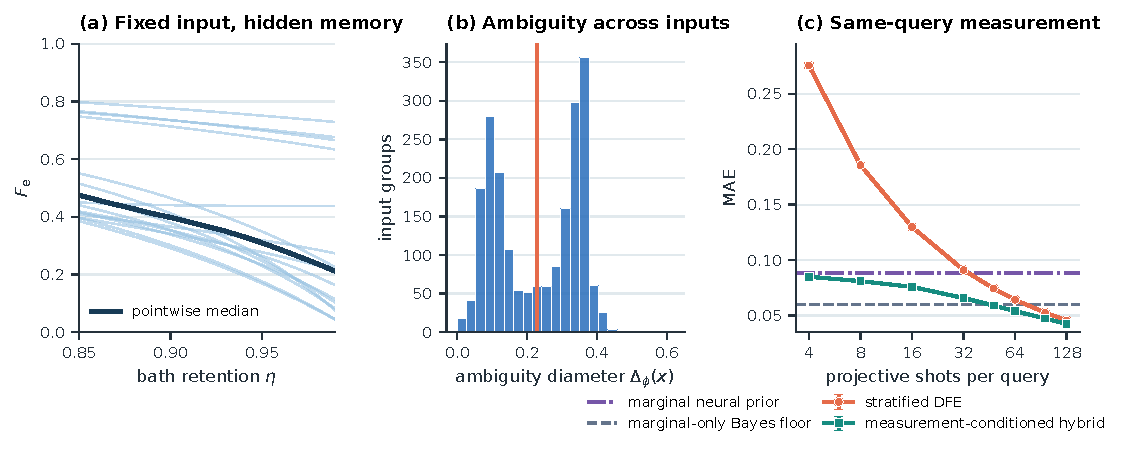
\includegraphics[width=0.98\textwidth]{identifiability_hybrid.pdf}
\caption{\textbf{Diagnosing and repairing missing information.} (a) Fixed marginal inputs can correspond to different fidelities as hidden bath retention varies. Curves show representative fibres. (b) The empirical ambiguity distribution yields a mean diameter of $0.229$, a mean pointwise minimax floor of $0.115$, and a uniform-$\eta$ Bayes MAE floor of $0.060$. (c) A same-query DFE pilot buys back the missing information: the neural hybrid reaches the accuracy of DFE with roughly one half to two thirds of its per-query shots in the highlighted regimes. Error bars show run-to-run standard deviations.}
\label{fig:identifiability_hybrid}
\end{figure*}

\paragraph*{Relation to architecture.}
The bidirectional transformer is used as the strongest marginal prior, but the effect is not architecture-exclusive: ridge and exact-marginal priors also benefit from fusion. The neural advantage is concentrated at small measurement budgets, where a better prior receives substantial weight. This is why we frame the contribution as an information-aware estimator rather than a new backbone.

\subsection{Two-qubit $d{=}4$ scaling}
\label{sec:exp_d4}

\Cref{tab:d4} reports results for the two-qubit order-sensitive regime. Here \fidno{}+cal improves over the product approximation by factors of $1.9$, $2.3$, and $1.8$ on \texttt{id\_test}, \texttt{length\_ood}, and \texttt{family\_ood}, respectively. The order-aware neural models also outperform the closed-form analytic baselines across the three splits.

This advantage does not extend to classical Monte-Carlo when a marginal simulation budget is available. MC with $K=100$ already reaches MAE $0.021$ on \texttt{id\_test}, and $K=1000$ reduces this to $0.007$, well below the neural models. Thus the $d=4$ experiment supports the regime interpretation rather than a general learned-surrogate advantage: neural predictors are appropriate when analytic formulas are too rough and per-query simulation or measurement is too costly, but Monte-Carlo remains preferable when marginal simulation is cheap enough.

\begin{table}[h]
\centering
\caption{\textbf{$d{=}4$ two-qubit order-sensitive: pooled MAE on $\Fe$.}}
\label{tab:d4}
\begin{tabular}{lccc}
\toprule
Method & \texttt{id\_test} & \texttt{length\_ood} & \texttt{family\_ood} \\
\midrule
Product approx.    & $0.110$ & $0.076$ & $0.091$ \\
FvG bound          & $0.238$ & $0.102$ & $0.218$ \\
\midrule
\fidno{} + cal     & $\bm{0.059 \pm 0.002}$ & $0.033 \pm 0.000$ & $0.051 \pm 0.001$ \\
\textsc{mlp} + cal & $0.075 \pm 0.001$ & $0.038 \pm 0.001$ & $0.060 \pm 0.001$ \\
\textsc{deepsets} + cal & $0.135 \pm 0.002$ & $0.038 \pm 0.001$ & $0.107 \pm 0.002$ \\
\textsc{bidir} + cal & $0.074 \pm 0.000$ & $\bm{0.032 \pm 0.001}$ & $0.055 \pm 0.002$ \\
\textsc{gnn} + cal & $0.077 \pm 0.003$ & $0.033 \pm 0.001$ & $0.047 \pm 0.001$ \\
\textsc{generic\_gnn} + cal & $0.072 \pm 0.003$ & $0.033 \pm 0.001$ & $\bm{0.039 \pm 0.002}$ \\
\midrule
MC, $K{=}10$       & $0.069$ & $0.056$ & $0.070$ \\
MC, $K{=}100$      & $0.021$ & $0.021$ & $0.022$ \\
MC, $K{=}1000$     & $0.007$ & $0.007$ & $0.007$ \\
\bottomrule
\end{tabular}
\end{table}

\paragraph*{Higher-dimensional regime pattern.}
The $d=4$ results show that closed-form analytic baselines lose accuracy as the channel family becomes richer and more order-sensitive. They also show the limit of the learned approach: when classical marginal Monte-Carlo is affordable, it is simpler and more accurate.

\paragraph*{GNN under family shift.}
The \textsc{generic\_gnn} model gives the best \texttt{family\_ood} MAE in this regime ($0.039$ versus $0.051$ for \fidno{}). We treat this as evidence that a path-graph inductive bias can help under some distribution shifts, but do not draw a broader architectural conclusion from a single split.
%%%% END flattened: sections/05_experiments

\subsection{Sample-complexity crossover}
\label{sec:exp_sample}

The comparison now has three Pareto points rather than a binary surrogate-versus-measurement choice. A marginal-only neural prior costs 4096 offline shots and no per-query shots but stops at MAE $0.0885$. Stratified DFE reduces error as $B^{-1/2}$. The measurement-conditioned hybrid occupies the gap: 32-shot hybrid and 64-shot DFE have comparable error ($0.0657$ versus $0.0641$), while 64-shot hybrid and 96-shot DFE are likewise close ($0.0539$ versus $0.0525$). Including both finite-shot labels and the independent pilots used to fit $w_B$, the offline costs are 6144 and 8192 shots. Consequently the total-shot curves cross after $6144/(64-32)=192$ and $8192/(96-64)=256$ deployment queries, respectively. Training-set simulation remains a separate classical cost in this benchmark.

\begin{figure}[h]
\centering
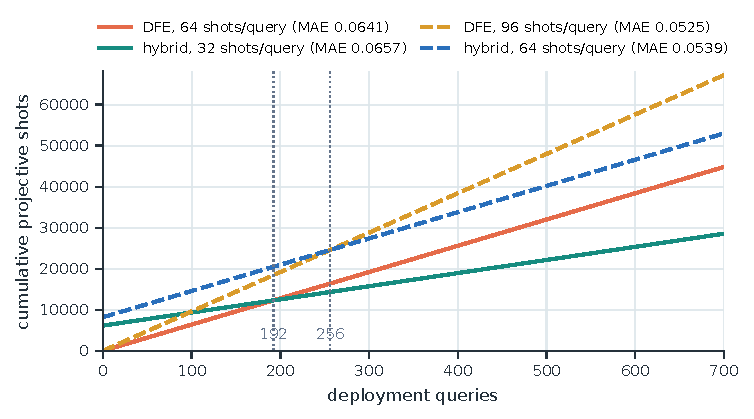
\includegraphics[width=0.78\linewidth]{break_even_queries.pdf}
\caption{\textbf{Full amortised measurement cost.} The build cost includes 64 independent 64-shot target labels and 64 independent $B$-shot fusion pilots. The 32-shot hybrid crosses 64-shot DFE after 192 queries at similar MAE; the 64-shot hybrid crosses 96-shot DFE after 256 queries.}
\label{fig:collision_amortised}
\end{figure}

\subsection{Wall-clock latency}
\label{sec:exp_latency}

\Cref{tab:latency} adds the deterministic baseline omitted from the original comparison. On the same server, direct superoperator composition of full Choi inputs is faster than the neural model for the single-qubit ID setting and of the same order for $d=4$. Exact composition remains numerically exact for the Markovian datasets. The timings use CPU for exact composition and GPU for neural inference and should not be read as a hardware-normalised speed contest; their purpose is to rule out a surrogate-speed claim for the studied small dimensions.

\begin{table}[h]
\centering
\caption{\textbf{Per-sequence wall-clock time (ms), $n\leq16$.} Exact composition uses CPU; neural inference uses one RTX 5090.}
\label{tab:latency}
\begin{tabular}{lc}
\toprule
Method & ms/sequence \\
\midrule
Product approximation & $0.0013\pm0.0003$ \\
Exact composition, $d=2$ & $0.150$ \\
\fidno{} (small), $d=2$ & $0.43\pm0.02$ \\
Exact composition, $d=4$ & $0.655$ \\
MC, $K{=}10$ & $3.45\pm0.10$ \\
MC, $K{=}100$ & $30.2\pm0.36$ \\
MC, $K{=}1000$ & $298.9\pm4.6$ \\
\bottomrule
\end{tabular}
\end{table}

\subsection{Distribution calibration: ECE and CRPS}
\label{sec:exp_calibration}

\Cref{tab:cal_metrics} reports distribution-quality metrics for the collision regime before the labelled-OOD affine correction used in \cref{tab:hybrid}. The MAE column is therefore the pre-affine point-prediction MAE, matching the raw \fidno{} row up to rounding, while ECE and CRPS evaluate the conformally adjusted quantile output. On the in-distribution split the quantile output achieves ECE $0.0042$ and CRPS $0.018$, close to the ideal calibration target. On length-OOD and family-OOD, however, the ID-fitted quantile correction does not transfer: ECE rises to $0.39$ and $0.50$ respectively, while CRPS deteriorates in line with the raw MAE. The separate labelled-OOD affine recalibration in \cref{tab:hybrid} corrects the mean MAE but does not recalibrate the full predictive distribution; we leave isotonic or conformal recalibration of the full OOD distribution to future work.

\begin{table}[h]
\centering
\caption{\textbf{Collision regime: pre-affine distribution metrics for \fidno{} (pooled over 5 seeds, $1024$ sequences).} MAE is the raw/pre-affine point error; ECE is measured on the predicted median band and CRPS over the nine-quantile output after ID-fitted quantile correction.}
\label{tab:cal_metrics}
\begin{tabular}{lccc}
\toprule
Split & MAE & ECE & CRPS \\
\midrule
\texttt{id\_test}      & $0.025$ & $\bm{0.004}$ & $0.018$ \\
\texttt{length\_ood}   & $0.138$ & $0.394$ & $0.119$ \\
\texttt{family\_ood}   & $0.383$ & $0.500$ & $0.359$ \\
\bottomrule
\end{tabular}
\end{table}
%%%% END flattened: sections/05_experiments


%%%% BEGIN flattened: sections/06_operating_regimes
\section{Operating Regimes and Implications}
\label{sec:operating}

The empirical pattern in~\cref{sec:experiments} yields a practical estimator-selection rule. The rule is based on a scaling argument and on the regimes studied here, so its numerical thresholds should be treated as calibration points rather than universal constants.

\subsection{The $\eps^{2} L^{2}$ scaling argument}

For a Pauli-diagonal channel $\Lset_i$ with infidelity
$\eps_i = 1-\Fe(\Lset_i)$, the product approximation expands as
\begin{equation}
1 - \Fhat^{\mathrm{prod}}(\Lset_{1:L})
\;=\;
1 - \prod_{i=1}^{L}(1-\eps_i)
\;=\;
\sum_{i=1}^{L}\eps_i
-
\sum_{i<j}\eps_i\eps_j
+
\mathcal{O}(\eps^{3}L^{3}).
\end{equation}
For Markovian compositions of Pauli-diagonal channels, the true infidelity shares the first-order term $\sum_i \eps_i$. Differences between the true composed fidelity and the product approximation therefore enter through pairwise and higher-order terms. At the pair level this discrepancy scales as
$\sum_{i<j}\eps_i\eps_j$, which is of order $\eps^2L^2$ when the per-channel infidelities are comparable.

For non-Markovian compositions, the same scaling serves only as a warning diagnostic. If consecutive channels are coupled through a shared bath, each pair of time steps can contribute a cross-correlation term. A marginal estimator has no representation of these terms, so the number of possible pair corrections still grows like $L^2$. We therefore use $\eps^2L^2$ only as an order-of-magnitude flag for when marginal factorisation should be stress-tested. Once $\eps$ is large or the bath coupling is non-perturbative, the expression is no longer a quantitative error estimate.

\paragraph*{Small $\eps$: hardware-like noise.}
In the device regime R1, $\eps \approx 10^{-3}$. At $L=16$, the diagnostic scale is $\eps^2L^2 \approx 2.5\times10^{-4}$, comparable to the residual error of the product approximation in our experiments. The correction that a learned model could recover is therefore smaller than the fitting error expected from a practical training set. This explains why the neural models do not improve over the analytic baseline. In this regime, the product approximation is the natural default, with direct measurement used when an unbiased experimental estimate is required.

\paragraph*{Large $\eps$: bath-mediated noise.}
In the collision regime R2, $\eps \approx 0.4$. At $L=16$, the diagnostic scale is no longer perturbatively small; it exceeds the fidelity range and should be read as a warning that marginal factorisation has broken down. In this setting, bath-mediated correlations can dominate the error of marginal estimators. This is the regime where a learned surrogate can help, provided the deployment distribution is covered by training or by labelled-OOD recalibration. In our experiments, calibrated sequence models improve strongly over uncalibrated marginal predictors, but stratified DFE matches their MAE with about 32 shots per query. Their defensible advantage is therefore zero-measurement inference after an offline calibration cost has been amortised, not superior attainable accuracy.

Thus, $\eps^2L^2$ is not a theorem-level error bound. It is a screening diagnostic: when it is small, there is little room for learning to improve on marginals; when it is large, marginal estimators should be stress-tested against correlated alternatives.

\subsection{Bath-retention sweep}

\Cref{fig:eta_sweep} tests this picture by sweeping the bath-retention parameter $\eta$ in the collision model. At $\eta=0$, the bath is reset and the marginal description is nearly valid; MC-1000 and the product approximation have MAE $0.009$ and $0.021$, respectively. As $\eta$ increases, the marginal estimators degrade quickly. At $\eta=0.85$, product and MC-1000 reach MAE $0.298$ and $0.318$, whereas \fidno{}+cal remains at $0.065$. At $\eta=0.99$, \fidno{}+cal still improves over the marginal estimators, but its MAE rises to $0.211$, indicating that this point lies near the edge of the calibrated training support.

\begin{figure}[h]
\centering
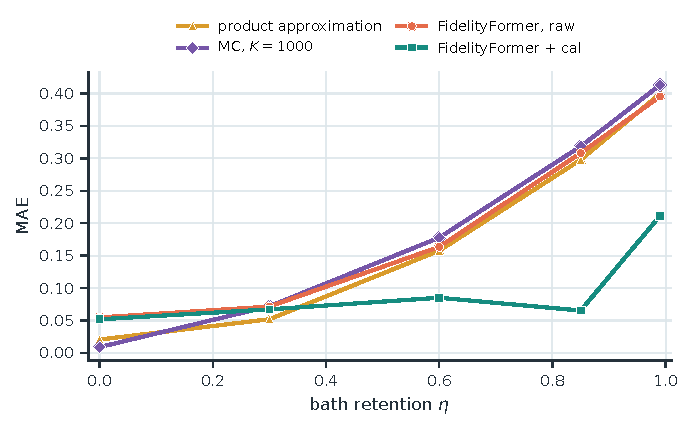
\includegraphics[width=0.72\linewidth]{eta_sweep.pdf}
\caption{\textbf{Bath-retention sweep for the decision rule.} Collision-regime MAE as the retention coefficient $\eta$ interpolates between Markovian marginals ($\eta=0$) and strong memory ($\eta \to 1$). Each point uses $1024$ sequences. Neural curves are averaged over five seeds; analytic and MC-1000 curves are evaluated on the same split.}
\label{fig:eta_sweep}
\end{figure}

\subsection{Decision rule}

\Cref{tab:decision} summarises the resulting rule of thumb. The thresholds are calibrated to our three regimes and to the $\eta$ sweep, and should be adjusted for other datasets.

\begin{table}[h]
\centering
\caption{\textbf{Operating-regime decision rule.}}
\label{tab:decision}
\begin{tabular}{p{0.34\linewidth}p{0.30\linewidth}p{0.26\linewidth}}
\toprule
Regime & Diagnostic signal & Recommended estimator \\
\midrule
Weak correlations / low infidelity
& $\eps^{2}L^{2} \lesssim 10^{-3}$
& Product approximation \\
Moderate correction, quantum shots affordable
& $10^{-3} \lesssim \eps^{2}L^{2} \lesssim 10^{-1}$
& \dfe{}, with shot budget matched to accuracy target \\
Marginals valid and classical simulation affordable
& $\eta \approx 0$ or validated Markovian marginals
& MC with $K \in [10^{2},10^{3}]$ \\
Strong memory, stable shift, and many measurement-free queries
& marginals fail; offline labels can be amortised
& calibrated low-capacity or neural surrogate \\
Strong memory without labels or shots
& large raw OOD bias expected
& raw surrogate only for ranking or triage, not absolute fidelity reporting \\
\bottomrule
\end{tabular}
\end{table}

The non-trivial cases are the middle and lower rows, where the deployment channel is correlated or non-Markovian. The choice is then a tradeoff among classical simulation cost, per-query quantum measurement cost, and one-time labelled characterisation cost. In our experiments, measurement-only DFE is the clean default when its required shot count is affordable, and a marginal-only prior is justified only when deployment measurements are prohibited. Between them, the conditioned hybrid reduces the shots needed for a target MAE by using the learned predictor as a shrinkage prior. It becomes cost-effective after the finite calibration expense is amortised over sufficiently many queries.

\subsection{QEC compatibility}

We do not claim that \fidno{} is a decoder, a threshold estimator, or a replacement for logical-error-rate estimation in QEC. It is better viewed as a proxy fidelity-estimation component in workflows where composed-channel quality must be queried repeatedly before committing to a more expensive decoder-level or experimental validation.

\begin{description}[itemsep=2pt,topsep=2pt,leftmargin=*]
\item[Logical-channel quality estimation.]
During code design, a logical-channel fidelity proxy can be useful for screening code patches or noise models. Our device regime suggests that, for low-infidelity Pauli-like noise, a learned surrogate is unlikely to improve on a calibrated analytic estimator. We do not infer logical error rates, decoder performance, or threshold behaviour from these fidelity estimates; those require separate decoder-level simulations or experiments.

\item[Memory cutoff and protocol selection.]
At higher infidelity, as in the collision regime, the practical question is often whether to keep, abort, or re-purify a noisy memory or partially purified state. In such settings, \fidno{}+cal can provide repeated fidelity estimates without consuming experimental shots, provided the deployment regime is fixed and labelled calibration data can be obtained offline.
\end{description}

In both cases, the surrogate complements existing QEC tools rather than replacing them. Its use is justified only when the cost of standard simulation or measurement is larger than the cost of building and amortising an offline labelled set.

\subsection{Scope and caveats}

Our claims are subject to four limitations.

\begin{enumerate}[itemsep=2pt,topsep=2pt,leftmargin=*]
\item \emph{Labelled-OOD calibration requires labels.}
The labelled calibration set ($N_{\mathrm{cal}}=64$ in the headline configuration, with a supplementary sweep down to $8$) must be obtained from exact simulation, an offline characterisation campaign, or another labelled-data source. The quantum or classical cost is paid once and amortised, but it is not free. We discuss unlabelled extensions, such as distribution matching at the predicted-quantile level, in~\cref{app:recalibration}.

\item \emph{The collision memory strength is not identifiable from the input.}
The reset-bath marginals are independent of $\eta$ for fixed collision parameters. Predictions therefore estimate a distribution-conditional correction; they do not reconstruct the realised bath state or per-sample retention coefficient.

\item \emph{The $d=4$ regime is not bath-mediated.}
The two-qubit channels in R3 are order-sensitive, but their correlations are coherent rather than environmental. Whether the recalibration behaviour observed in R2 extends to genuinely bath-mediated systems with $d>2$ remains open.

\item \emph{The architecture is not the main claim.}
\fidno{} is one member of a broader class of causal sequence models. Across our experiments, several learned backbones reach comparable accuracy within seed variation. The main contribution is the operating-regime characterisation and the calibration-based deployment picture, not a claim that this particular architecture is uniquely optimal.
\end{enumerate}
%%%% END flattened: sections/06_operating_regimes


%%%% BEGIN flattened: sections/07_related
\section{Related work}
\label{sec:related}

\paragraph*{Fidelity-estimation tools.}
The estimators compared in~\cref{sec:baselines} are standard tools in quantum information. Product-style approximations appear in analyses of repeater chains and quantum-network protocols~\cite{repeater_review}. Direct Fidelity Estimation~\cite{flammia_liu_2011} estimates fidelity through Pauli measurements on the implemented channel. Randomised benchmarking~\cite{rb_review,rb_recent} estimates Clifford-averaged gate fidelity, while cross-entropy benchmarking~\cite{xeb_review} provides a related sequence-level diagnostic. Diamond-norm semidefinite programs~\cite{watrous_dnorm_sdp,khatri_dnorm} give worst-case channel-distance estimates, at substantially higher classical cost.

\paragraph*{Learned surrogates for scientific computation.}
Learned surrogates that replace an expensive numerical estimator with a fast forward model are now widespread across the sciences. Operator-learning architectures such as the Fourier Neural Operator~\cite{fno} and DeepONet~\cite{deeponet} approximate solution maps of parametric differential equations and have become standard tools in scientific machine learning. A recurring question in this literature is not which architecture is largest, but when a surrogate is trustworthy enough to replace the estimator it approximates, and how its error behaves out of distribution. Our study is an instance of this question for a composed-estimator prediction task: rather than proposing a new operator architecture, we characterise the operating regimes in which a learned surrogate is preferable to the analytic, sampling, or measurement-based estimator it is meant to replace, and quantify the labelled-calibration cost of closing the out-of-distribution gap.

\paragraph*{Learned channel-fidelity surrogates.}
Neural surrogates have been used for quantum-dynamics prediction, dissipative evolution, and Lindbladian learning~\cite{nn_channel_seq,nn_supop}. Quantum-aware graph networks and equivariant variants have also been explored for quantum-network estimation~\cite{deepsets_channels,gnn_channels}. In the repeater setting, related work includes reinforcement-learning agents for protocol selection~\cite{nn_repeater} and Bayesian-optimisation approaches to protocol search~\cite{repeater_BO_external}. Our focus is different: we ask when a learned surrogate is preferable to analytic, Monte-Carlo, or measurement-based estimators, and when it is not.

\paragraph*{Non-Markovian collision models.}
Collision models are widely used to study non-Markovian open-system dynamics~\cite{ciccarello_collision_review,collision_app}. Prior work mainly uses them as forward-simulation models. Here we use a collision-model family as a stress test for fidelity estimators that only see marginal channel information.

\paragraph*{Distribution shift and post-hoc calibration.}
Post-hoc calibration methods such as affine, temperature, and isotonic calibration are standard in classification and probabilistic regression~\cite{guo_calibration,kuleshov_calibrated}. Our labelled-OOD calibration setting is closer to bias correction than to classical coverage calibration: the goal is to remove a systematic shift in the median fidelity prediction. Conformal prediction~\cite{conformal_review} could be used to calibrate predictive intervals for $\Fe$ and is a natural extension.

\paragraph*{Surrogate-driven QEC code design.}
Learned surrogates have recently been proposed inside QEC code-design loops as inner-loop fidelity proxies~\cite{qec_surrogate}. Our results suggest a regime-dependent interpretation of such methods, but not a decoder-level or threshold-level claim. In low-infidelity Pauli-like regimes, analytic estimators may already be near-optimal; learned surrogates become more relevant when correlated noise produces corrections that marginal estimators cannot represent.
%%%% END flattened: sections/07_related


%%%% BEGIN flattened: sections/08_conclusion
\section{Conclusion}
\label{sec:conclusion}

The central question in scientific surrogate modelling is not whether a network can fit a target, but whether the target is identifiable from the variables available at inference and whether a cheaper estimator already exists. For composed quantum-channel fidelity, exact superoperator composition settles the complete Markovian case, while stratified DFE settles many measurement-rich cases.

The remaining non-Markovian setting is genuinely information-limited. Our paired counterfactual audit turns that statement into a measurable certificate: unchanged marginal inputs support a mean fidelity range of $0.229$, with a uniform-high-memory Bayes MAE floor of $0.060$. This identifies which residual errors no marginal-only architecture can remove. A small measurement on the same query then repairs the information contract. Convex prior--DFE fusion matches 64-shot DFE using 32 shots and matches 96-shot DFE using 64 shots on an independent-random-stream split, with full calibration costs amortised after 192 and 256 queries.

These results support a disciplined workflow: compose when the supplied channel descriptions are complete, measure when the deployed process is accessible, use a learned prior only under a stable repeat-query contract, and combine prior and measurement when each alone lies off the desired cost--accuracy frontier. More broadly, counterfactual representation audits and measurement-conditioned fusion provide a route to novelty in scientific machine learning that is based on information and decision value rather than architectural complexity.

\section*{Author contributions}

 SW and XL contributed equally to this work. SW and XL conceived the study, developed the methodology, performed the experiments, analysed the results, and prepared the figures and tables. SW drafted the manuscript. WY supervised the project, guided the interpretation and framing of the results, and revised the manuscript. All authors discussed the results, commented on the manuscript, and approved the final version.

\section*{Competing interests}

All authors declare no financial or non-financial competing interests.

\section*{Data availability}

All datasets are generated synthetically by the scripts in the public repository, \url{https://github.com/shchng9963-droid/fidelityno}. Versioned generated-data and result archives will be deposited with an archival DOI before acceptance; the submission bundle records the exact code revision and random seeds.

\section*{Code availability}

The underlying code for this study is available in Github and can be accessed via this link \url{https://github.com/shchng9963-droid/fidelityno}.

\section*{Use of AI and AI-assisted technologies}

LLMs were used to improve grammar, wording, and readability of the manuscript text.

\bibliographystyle{iopart-num}
\bibliography{bibliography}

\newpage

\appendix

%%%% BEGIN flattened: appendices/A_pauli_saturation
\section{First-order accuracy of the product approximation for Pauli-diagonal channels}
\label{app:pauli}

We sketch why the product approximation~\eqref{eq:product_approx} is first-order accurate when each per-channel marginal $\Lset_i$ is Pauli-diagonal in a common basis, which is the configuration realised by our IBM \texttt{Fake*V2} noise-model regime to leading order. The result we use is a scaling argument $\Fhat^{\mathrm{prod}}_{\mathrm{err}} = \mathcal{O}(\eps^{2} L^{2})$, not a saturation theorem.

Let $\Lset_i$ act as a Pauli channel,
\begin{equation}
\Lset_i(\rho) \;=\; \sum_{P \in \{I, X, Y, Z\}^{\otimes \log_2 d}} p_{i,P} \, P \rho P^{\dagger},
\end{equation}
with $\sum_P p_{i,P} = 1$. The Choi matrix $\Choi(\Lset_i)$ is then diagonal in the Pauli basis, and the entanglement fidelity reduces to the identity weight $\Fe(\Lset_i) = p_{i, I}$.

Composition $\Lset_{1:n} = \Lset_n \circ \cdots \circ \Lset_1$ produces another Pauli channel. The identity weight of the composed channel is \emph{not} in general equal to the product $\prod_{i} p_{i, I}$ of identity weights: contributions of the form $P P P P \cdots = I$ for the same Pauli $P$ at multiple positions, and triple-products $P_1 P_2 P_3 = I$, also land in the identity bucket. Counting cross-channel pair contributions of $(P, P)$ for $P \neq I$ at any pair of positions gives a correction
\begin{equation}
p_{1:n,I}-\prod_{i=1}^{n}p_{i,I}=\sum_{i<j}\sum_{P\neq I}p_{i,P}p_{j,P}\!\prod_{k\neq i,j}p_{k,I}+\mathcal{O}(L^{3}\eps^{3}).
\end{equation}
Each summand is $\mathcal{O}(\eps^{2})$ and there are $\binom{n}{2}$ pairs, giving a leading-order correction of order $\eps^{2} L^{2}$ where $L = n$ and $\eps$ is the typical per-channel infidelity. The product approximation is therefore first-order accurate in $\eps$ but acquires a $\eps^{2} L^{2}$ correction at second order.

When the channels are not Pauli-diagonal in a common basis, an additional ``Pauli-rotation'' correction arises but it remains $\mathcal{O}(\eps^{2})$ at leading order. The collision-model regime exhibits a much larger correction because the dynamics are not Pauli at all, and the bath-mediated terms are $\mathcal{O}(\eta)$ rather than $\mathcal{O}(\eps^{2})$; this is what the surrogate learns to recover.

We do not require this scaling for any of the experimental claims in the main text; it is included here to clarify the precise scope of the ``product approximation is near-exact'' statement in (R1).
%%%% END flattened: appendices/A_pauli_saturation


%%%% BEGIN flattened: appendices/B_recalibration
\section{Affine recalibration across random seeds}
\label{app:recalibration}

\Cref{tab:recal_seeds} reports a separate legacy audit in which per-seed affine $(a, b)$ coefficients were fitted on a labelled, held-out 10\% subset of the collision \texttt{family\_ood} (memory-strength-OOD) data. Its calibration set and split realisation differ from the fixed $N_{\mathrm{cal}}=64$ counterfactual audit in \cref{tab:ambiguity}, so its mean MAE of $0.094$ should not be used as a paired comparison with the headline $0.090$. Within this audit, the five seeds reach similar calibrated MAE (std $1.3 \times 10^{-3}$) despite variation in the fitted affine coefficients (slope std $\approx 0.09$), indicating that the slope and intercept are correlated and should not be interpreted separately.

\begin{table}[h]
\centering
\caption{\textbf{Affine recalibration coefficients, \fidno{} on collision \texttt{family\_ood}.} 5 seeds, 10\% OOD calibration set. The fitted slope is $a$ and intercept is $b$ in $\Fhat^{\mathrm{cal}} = a \Fhat^{\mathrm{raw}} + b$.}
\label{tab:recal_seeds}
\begin{tabular}{ccccc}
\toprule
seed & $a$ & $b$ & MAE raw & MAE cal \\
\midrule
0 & $2.845$ & $-1.916$ & $0.387$ & $0.095$ \\
1 & $2.822$ & $-1.896$ & $0.386$ & $0.095$ \\
2 & $2.918$ & $-1.980$ & $0.387$ & $0.094$ \\
3 & $3.026$ & $-2.080$ & $0.388$ & $0.095$ \\
4 & $3.003$ & $-2.052$ & $0.387$ & $0.092$ \\
\midrule
mean   & $2.923$ & $-1.985$ & $0.387$ & $0.094$ \\
std    & $0.091$ & $0.081$ & $0.001$ & $\bm{0.001}$ \\
\bottomrule
\end{tabular}
\end{table}

\paragraph*{Seed-to-seed variation in affine coefficients.}
The $\sim 0.1$ variation in the slope $a$ does not translate into comparable variation in test MAE because slope and intercept co-vary over the narrow range of raw predictions. The result supports reporting predictive error across seeds, but it does not by itself identify the physical source of the OOD bias.

\paragraph*{Quantile calibration.}
We apply the same affine $(a, b)$ to all $K = 9$ predicted quantile levels, which preserves quantile monotonicity but not necessarily empirical coverage on OOD. In our experiments quantile coverage is recovered to within $\pm 0.04$ of nominal at the medium-to-high quantiles ($q \geq 0.5$); coverage at low quantiles ($q \leq 0.3$) is occasionally over-coverage on \texttt{family\_ood} due to clipping at $\Fe = 0$. A more principled extension would fit a per-quantile shift, which we leave to future work.

%%%% END flattened: appendices/B_recalibration


%%%% BEGIN flattened: appendices/C_implementation
\section{Implementation details}
\label{app:implementation}

\paragraph*{Software and numerical backends.}
PyTorch 2.6 + CUDA 12.8 (RTX 5090, sm\_120). Differentiable simulator: \texttt{dynamiqs} 0.3 for time-dependent Lindblad evolution, with \texttt{qutip} 5.2 used for cross-validation of Choi matrices to a tolerance of $10^{-8}$. Diamond-norm SDP via \texttt{cvxpy} 1.9.1 wrapping the SCS solver, called through \texttt{qutip.dnorm} for production runs. Hydra for configs; \texttt{wandb} for offline logging.

\paragraph*{Model architecture.}
\fidno{}: $d_{\mathrm{model}} = 256$, depth 6, heads 8, FFN expansion $4\times$, rotary positional encoding, GELU non-linearity, dropout $0.1$. Channel encoder: 2-layer MLP, hidden dim 512, GELU. Quantile head: $K = 9$ levels at $\{0.1, 0.2, \ldots, 0.9\}$, softplus output, bias initialised so that the median quantile starts at $\Fe \approx 0.7$ (essential to avoid dead-gradient saturation in the deep-circuit regime). Auxiliary physics-consistency head: 2-layer MLP, $0.1$ weight on auxiliary loss.

\paragraph*{Training protocol.}
AdamW, lr $3 \times 10^{-4}$, cosine decay to $10^{-5}$, weight decay $10^{-2}$. 80 epochs, batch size 256 (collision and $d{=}4$), batch size 128 (device regime). Early-stopping patience 20. We apply a length curriculum: starting epochs sample lengths $\in \{2, 4\}$ uniformly, expanding to $\{2, 4, 8, 16\}$ over the first 30 epochs.

Architecture and training hyperparameters were selected on the calibration split of the device regime and held fixed across regimes. We did not run a per-regime sweep, which we view as a stress test of the architecture's regime-agnosticity.

\paragraph*{Dataset splits.}
Each split contains $8{,}000$ sequences (collision, $d{=}4$) or $1{,}024$ sequences per backend (device). Lengths are sampled from $\{2,4,8,16\}$ for train/calib/id\_test and $\{24,32,48\}$ for length\_ood. In the collision data, the legacy family\_ood filename denotes a held-out $\eta\in[0.85,0.99]$ interval; training uses $\eta\in[0,0.7]$. Random seeds are disjoint across splits.

\paragraph*{Reproducibility and validation.}
The five seeds are $\{0, 1, 2, 3, 4\}$, applied to (a) NumPy / PyTorch global RNG, (b) channel parameter sampling, (c) train/val/test split assignment, (d) model initialisation, (e) data shuffling. The 84 unit tests cover CPTP sanity for every channel-family generator, Choi composition associativity, quantile-head monotonicity, recalibration coefficient stability, diamond-SDP correctness against a QuTiP reference, and an end-to-end smoke-train on a 100-sample subset. Total wall-clock for a fresh reproduction on a 2$\times$ RTX 5090 setup: $\sim 5$ hours, dominated by neural training.

%%%% END flattened: appendices/C_implementation

\end{document}
